\documentclass[10pt,a4paper]{article}

\usepackage[T1]{fontenc}
\usepackage[utf8]{inputenc}
\IfFileExists{lmodern.sty}{\usepackage{lmodern}}{\usepackage[scaled=.95]{helvet}}
\usepackage[expansion=false]{microtype}
\usepackage[a4paper,left=18mm,right=18mm,top=25mm,bottom=20mm,headheight=17mm,headsep=8mm,footskip=10mm]{geometry}
\usepackage{xcolor}
\usepackage{graphicx}
\usepackage{tabularx}
\usepackage{array}
\usepackage{booktabs}
\usepackage{enumitem}
\usepackage{titlesec}
\usepackage[most]{tcolorbox}
\usepackage{fancyhdr}
\usepackage{lastpage}
\usepackage{tikz}
\usepackage{hyperref}
\hypersetup{hidelinks}
\usepackage[backend=biber,style=ieee,sorting=none]{biblatex}
\addbibresource{../ref.bib}

% -----------------------------------------------------------------------------
% Colours sampled/approximated from the original document
% -----------------------------------------------------------------------------
\definecolor{MetroBlue}{HTML}{23477F}
\definecolor{MetroOrange}{HTML}{F39200}
\definecolor{BodyText}{HTML}{202B3A}
\definecolor{Muted}{HTML}{65748A}
\definecolor{RuleGray}{HTML}{D3D6DA}
\definecolor{PanelGray}{HTML}{F1F2F4}
\definecolor{ConfRed}{HTML}{C9252B}

\color{BodyText}
\setlength{\parindent}{0pt}
\setlength{\parskip}{0pt}
\renewcommand{\familydefault}{\sfdefault}

% -----------------------------------------------------------------------------
% Header and footer
% -----------------------------------------------------------------------------
\newcommand{\ConfidentialBox}{%
  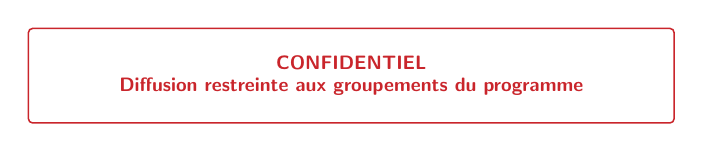
\begin{tikzpicture}[baseline=(current bounding box.center)]
    \node[draw=ConfRed, rounded corners=1.5pt, line width=.55pt,
      minimum width=82mm, minimum height=12mm, align=center,
      text=ConfRed, font=\bfseries\fontsize{6.7}{8}\selectfont, inner sep=2pt]
      {CONFIDENTIEL\\Diffusion restreinte aux groupements du programme};
  \end{tikzpicture}%
}
\pagestyle{fancy}
\fancyhf{}
\fancyhead[L]{\raisebox{1.5mm}{\color{Muted}\fontsize{7.2}{8.5}\selectfont
  Metropolis $\cdot$ Programme Renouvellement Signalisation $\cdot$ OM}}
\fancyhead[R]{\ConfidentialBox}
\fancyfoot[R]{\color{Muted}\fontsize{7.5}{9}\selectfont\thepage\,/\,\pageref{LastPage}}
\renewcommand{\headrulewidth}{0pt}
\renewcommand{\footrulewidth}{0pt}

% -----------------------------------------------------------------------------
% Section heading style
% -----------------------------------------------------------------------------
\titleformat{\section}
  {\normalfont\bfseries\Large\color{MetroBlue}}
  {\textcolor{MetroOrange}{\thesection.}}{0.55em}{}
\titlespacing*{\section}{0pt}{0pt}{8pt}

% Action/expectation procedure panels
\newtcolorbox{procedurebox}{
  colback=PanelGray,
  colframe=PanelGray,
  boxrule=.45pt,
  arc=2mm,
  left=4mm,right=4mm,top=2.5mm,bottom=2.5mm,
  before skip=8pt, after skip=0pt
}

\newlist{teststeps}{enumerate}{1}
\setlist[teststeps]{label=\arabic*., leftmargin=6mm, labelsep=2mm,
  itemsep=3.3pt, topsep=3pt, parsep=0pt, partopsep=0pt}
\newlist{substeps}{enumerate}{1}
\setlist[substeps]{label=\alph*., leftmargin=7mm, labelsep=2mm,
  itemsep=3pt, topsep=3pt, parsep=0pt, partopsep=0pt}


% Object-type cards ----------------------------------------------------------
\newcommand{\lab}[1]{\textcolor{Muted}{#1}}
\newtcolorbox{typecard}[1]{
  enhanced, breakable=false,
  colback=white, colframe=RuleGray, boxrule=.45pt, arc=1.2mm,
  borderline west={2.2pt}{0pt}{MetroBlue},
  left=4mm,right=3mm,top=2mm,bottom=1.5mm,
  before skip=6pt, after skip=4pt,
  title={}, fonttitle=\bfseries,
  before upper={{\bfseries\color{MetroBlue}\normalsize #1\par}\vspace{1.5mm}}
}
\newenvironment{typerows}
  {\renewcommand{\arraystretch}{1.25}\small
   \begin{tabular}{@{}>{\raggedright\arraybackslash}p{0.14\linewidth}>{\raggedright\arraybackslash}p{0.82\linewidth}@{}}}
  {\end{tabular}}
\newcommand{\para}[1]{\par\vspace{1mm}#1\par\vspace{2mm}}

\begin{document}
\thispagestyle{fancy}

\vspace*{1mm}
\noindent
\begin{minipage}[c]{0.59\textwidth}
  
\includegraphics[height=1.4cm,keepaspectratio]{../logo/LogoMetropolis.pdf}
\end{minipage}%
\begin{minipage}[c]{0.40\textwidth}
  \raggedleft
  
\includegraphics[height=0.45cm,keepaspectratio]{../logo/LogoProver.pdf}
\end{minipage}

\vspace{12mm}
{\color{MetroOrange}\bfseries\fontsize{8.2}{10}\selectfont
  P R O G R A M M E\quad R E N O U V E L L E M E N T\quad S I G N A L I S A T I O N\par}

\vspace{4mm}
{\color{MetroBlue}\bfseries\fontsize{25}{30}\selectfont
  Object model for Metropolis GA\\[-1mm]
  package\par}

\vspace{2mm}
{\color{Muted}\fontsize{10.5}{13}\selectfont Version 0.3, 2026-11-06\par}

\vspace{10mm}
{\color{Muted}\bfseries\fontsize{7.5}{9}\selectfont REVISION HISTORY\par}
\vspace{2mm}
\renewcommand{\arraystretch}{1.55}
\begin{tabularx}{\textwidth}{@{}>{\raggedright\arraybackslash}p{0.13\textwidth}
  >{\raggedright\arraybackslash}p{0.17\textwidth}
  >{\raggedright\arraybackslash}p{0.13\textwidth}
  >{\raggedright\arraybackslash}X@{}}
  \textcolor{Muted}{\bfseries\fontsize{7}{8}\selectfont VERSION} &
  \textcolor{Muted}{\bfseries\fontsize{7}{8}\selectfont DATE} &
  \textcolor{Muted}{\bfseries\fontsize{7}{8}\selectfont AUTHOR} &
  \textcolor{Muted}{\bfseries\fontsize{7}{8}\selectfont CHANGE} \\
  \midrule
  0.1 & 2022-06-15 & DF & Draft version for review \\
  \midrule
  0.2 & 2022-10-25 & HF & Adding exit signals and buffer stops \\
  \midrule
  0.3 & 2026-11-06 & G & Adding manual release of routes (Release Requested, Release Timer, Just Unlocked) \\
  \bottomrule
\end{tabularx}

\vspace{4mm}
\begin{tcolorbox}[
  colback=PanelGray,colframe=PanelGray,boxrule=0pt,arc=2mm,
  left=4mm,right=4mm,top=3mm,bottom=2.5mm]
  {\color{Muted}\bfseries\fontsize{7.5}{9}\selectfont CONTENTS\par}
  \vspace{2mm}
  \begin{enumerate}[label=\textcolor{MetroOrange}{\bfseries\arabic*.},
    leftmargin=5mm,labelsep=2mm,itemsep=2.5mm,topsep=0pt,parsep=0pt]
    \item Introduction
    \item Object types
  \end{enumerate}
\end{tcolorbox}

\newpage

\section{Introduction}
This is the informal object model for the Metropolis GA package.

Object types used are tracks, signals, exit signals, buffer stops, route sections, routes, switches and protection areas.

\vspace{6mm}
\section{Object types}

\begin{typecard}{Type: Track}
\begin{typerows}
\lab{Inputs} & Clear (from occupancy) \\
\lab{Outputs} & - \\
\lab{Internal} & - \\
\lab{Relations} & - \\
\lab{Defined} & - \\
\end{typerows}
\end{typecard}
The input Clear represents the input from the detection device that is assumed to be present for each track.

\begin{typecard}{Type: Signal}
\begin{typerows}
\lab{Inputs} & Shows Proceed \\
\lab{Outputs} & Commanded Proceed \\
\lab{Internal} & - \\
\lab{Relations} & - \\
\lab{Defined} & End Locked := the Signal is End Signal to a Route whose Last Route Section is Locked. \\
\end{typerows}
\end{typecard}
The input Shows Proceed represent the input from the signal that confirms that the signal is actually showing a proceed aspect. The output Commanded Proceed represents the output that commands the signal to show proceed. Typically, the signal is optical, lighting particular lamps in order to show proceed and Commanded Proceed tells the signal to light those lamps. The defined state End Locked indicates that the signal might be in need of front protection.

\begin{typecard}{Type: Exit Signal}
\begin{typerows}
\lab{Inputs} & Shows Proceed, Line Input \\
\lab{Outputs} & Commanded Proceed, Line Output \\
\lab{Internal} & - \\
\lab{Relations} & - \\
\lab{Defined} & End Locked := the Signal is End Signal to a Route whose Last Route Section is Locked. \\
\end{typerows}
\end{typecard}
In addition to the I/Os of a normal signal, exit signals have an output that is sent to the neighbouring interlocking and an input received from the neighbouring interlocking. The output Line Output indicates that this exit signal is not Commanded Proceed and not End Locked. The Line Output is to be connected to the Line Input of the exit signal at the other end of the line, and vice versa.

\begin{typecard}{Type: Buffer Stop}
\begin{typerows}
\lab{Inputs} & - \\
\lab{Outputs} & - \\
\lab{Internal} & - \\
\lab{Relations} & - \\
\lab{Defined} & - \\
\end{typerows}
\end{typecard}
Buffer stops are passive objects that are possible end objects for routes.

\begin{typecard}{Type: Switch}
\begin{typerows}
\lab{Input} & Detected Normal, Detected Reverse, Request Normal, Request Reverse \\
\lab{Output} & Move Normal, Move Reverse \\
\lab{Internal} & Commanded Normal, Commanded Reverse \\
\lab{Relations} & - \\
\lab{Defined} & - \\
\end{typerows}
\end{typecard}
Switches can be in either normal (normally straight) or reverse (normally bent) positions. The inputs Detected Normal and Detected Reverse represents the inputs from the detection devices that are assumed to be present for each switch. The inputs Request Normal and Request Reverse represents inputs from the office system, used to change position of the switch. The internal states Commanded Normal and Commanded Reverse keeps track of the position that the interlocking expects the switch to be in. The outputs Move Normal and Move Reverse represent the outputs to the device that changes the position of the switch, usually an electrical motor.

\vspace{2mm}
As explained earlier, locked routes are the main concept used in order to inhibit collisions. Routes should be locked as a whole. However, in order to make it possible to unlock, or release, routes in bits, routes are divided into route sections. Both these types are of an abstract kind in the sense that they don't represent something physically present in the railyard.

\begin{typecard}{Type: Route Section}
\begin{typerows}
\lab{Inputs} & - \\
\lab{Outputs} & - \\
\lab{Internal} & Locked, Ready To Release \\
\lab{Relations} & Switch In Normal Position (Route Section, Switch), Switch In Reverse Position (Route Section, Switch), Tracks (Route Section, Track) \\
\lab{Defined} & - \\
\end{typerows}
\end{typecard}
The internal state Locked represents that the section is locked and the internal state Ready To Release represents that the section is ready to release. At this stage, these states does not have much meaning attached to them. That will be provided by the requirements. The relations Switch In Normal/Reverse Position give exactly those switches that need to be in normal/reverse position in order for the section to be traversable for a train. The relation Tracks gives the tracks that are contained in the section. In addition to being released when a train has passed it, a route section is unlocked when a route that contains it is manually released (see Just Unlocked in the type Route).

\begin{typecard}{Type: Route}
\begin{typerows}
\lab{Inputs} & Request Route, Release Requested \\
\lab{Outputs} & - \\
\lab{Internal} & Release Timer \\
\lab{Relations} & Route Sections (Route, Route Section), Start Signal (Route, Signal), End Object (Route, Signal/Exit Signal/Buffer Stop), Last Route Section (Route, Route Section) \\
\lab{Defined} & Set := all Route Sections are Locked and the Release Timer is not running \newline
Just Unlocked := the Release Timer was running in the previous cycle and is not running now, or Immediate Manual Release \newline
Immediate Manual Release := false \\
\end{typerows}
\end{typecard}
The input Request Route represents an input from the office system. It is used to lock all the route sections in the route and then, if permitted, clear the starting signal. The defined state Set simply states that a route is considered to be set when all its route sections are locked and the release timer is not running. The relation Route Sections gives the route sections that are contained in the route. The relations Start/End Signal give the facing signals that are assumed to be placed at the start/end of the route.

\para{The input Release Requested represents a request from the office system for manual release of the route. The release is done with a delay, giving any train that is traveling through the route or approaching it a fair chance to come to a stop. When Release Requested is received for a locked route, the Release Timer starts running (unless Immediate Manual Release holds). While it runs the route is not Set, so the start signal is no longer commanded to proceed. The timer stops 30 seconds after it started, whereupon Just Unlocked unlocks all route sections of the route simultaneously. Immediate Manual Release is a hook for releasing without delay; in the generic application it is always false.}

\end{document}